\section{Experiment}
\label{sec:experiment}
In this section, we proceed to introduce the experimental settings and results. Our GPU device is Tesla P100 with 16GB memory. We use python 3.7 based Keras to implement all the experiments.

\subsection{Datasets and Baselines}
\label{sec:dataset}
The datasets of our experiment are  PHEME \cite{DBLP:conf/coling/KochkinaLZ18} and RumorEval \cite{DBLP:conf/semeval/EnayetE17}. These two datasets are widely used in the rumor detection research area. The details of PHEME are shown in Table.\ref{tab:pheme} and the details of RumorEval are shown in Table.\ref{tab:RumorEval}. The original PHEME contains 9 events and 4 of them are sparse, so we usually use PHEME-5 (following the existing works \cite{DBLP:conf/www/ChengNB20}). The PHEME-5 is formed by the top-5 scaled events, which contains 5802 threads and 1972 in them are rumors. 

To demonstrate the effectiveness of RL-BRT, we choose baselines as comparisons, including (Naive Bayes, SGD, Dense, BiLSTM) \cite{DBLP:conf/emnlp/QazvinianRRM11}, FastText\cite{DBLP:conf/eacl/GraveMJB17}, TextCNN\cite{DBLP:conf/emnlp/Kim14}, VRoC \cite{DBLP:conf/www/ChengNB20}, and some combinations of them. All the chosen baselines are contained in Table.\ref{tab:results_RE}. We use accuracy and macro-F1 as the evaluation metrics.

\begin{table}[htbp]
	\caption{PHEME}
	\centering
	\label{tab:pheme}
	\resizebox{0.8\linewidth}{!}{
		\begin{tabular}{|c|c|c|c|}
			\hline
			\textbf{Events} & \textbf{Threads} & \textbf{Tweets} & \textbf{Threads of Rumors}\\
			\hline
			Charlie Hebdo (C) &2079&38268&458\\
			\hline
			Sydney siege (S) &1221&23996&522\\
			\hline
			Ferguson (F) &1143&24175&284\\
			\hline
			Ottawa Shooting (O) &890&12284&470\\
			\hline		
			Germanwings-crash (G) &469&4489&238\\
			\hline
			\textbf{Total} & 5802 & 103212 & 1972 \\
			\hline	
		\end{tabular}
	}	
\end{table}

\begin{table}[htbp]
	\caption{RumorEval}
	\centering
	\label{tab:RumorEval}
	\resizebox{0.6\linewidth}{!}{
		\begin{tabular}{|c|c|c|c|}
			\hline
			\textbf{}  & \textbf{Threads} & \textbf{Branch} & \textbf{Tweets}\\
			\hline
			Development  &25&215&281\\
			\hline
			Testing  &28&772&1049\\
			\hline
			Training &272&3030&4238\\
			\hline	
			\textbf{Total}  &325 &4017 &5568 \\
			\hline		
		\end{tabular}
	}	
\end{table}


\subsection{Experimental Results}
The results on RumorEval are shown in Table.~{\ref{tab:RumorEval}}. The second column records the F1-Scores on each event, and ``F, O, S, C, G" are the first chars of the corresponding event name. The plus ``+'' means we aggregate models by adding the output vectors after softmax. The results suggest that RL-BRT achieves the best performance on both average accuracy and average F1-Score. TextCNN achieves the best performance among these basic models. It is because the bag-of-words idea in TextCNN is suitable for the short text and various filters with different length effectively capture the features of key grams. Naive Bayes achieves the worst performance. We think the reason is that the parameters in Naive Bayes are limited, which is not enough for this corpus. SGD+TextCNN achieves the best performance among the pairwise-added models. 

The results on PHEME are shown in Table.~\ref{tab:results_PHE}. It suggests that RL-BRT model achieves the best performance on average accuracy and average macro-F1 score. The SGD achieves the worst performance among all basic models. We think it is because the scale of PHEME is larger than that of the RumorEval, and the SGD is not suitable for large-scale datasets. For F1-Score on every event, RL-BRT achieves the best performance on all events. To sum up, RL-BRT achieves excellent performance on all datasets, which demonstrates the effectiveness.A

\begin{table}[htbp]
	\caption{Results on RumorEval}
	\centering
	\label{tab:results_RE}
	\resizebox{1\linewidth}{!}{
		\begin{tabular}{|c|c|c|c|}
			\hline
			\multirow{2}{*}{\textbf{Methods}}  & \textbf{F1-Score on each event} & \multirow{2}{*}{\textbf{Average Accuracy}} & \multirow{2}{*}{\textbf{Average Macro-F1}}\\
			& \textbf{F/ O/ S/ C/ G} &  & \\
			\hline
			NB  & 0.937/0.924/0.907/0.929/0.617 & 0.910 & 0.863\\
			\hline
			SGD  & 0.977/0.964/0.942/0.928/0.927 & 0.950 & 0.948\\
			\hline
			FastText & 0.973/0.944/0.927/0.905/0.954
			& 0.938 & 0.940 \\
			\hline	
			Dense  & 0.964/0.951/0.939/\textbf{0.937}/0.919
			&0.946 &0.942 \\
			\hline
			BiLSTM  & 0.972/0.909/0.910/0.895/0.901
			&0.920 &0.917 \\
			\hline
			TextCNN  & \textbf{0.991}/\textbf{0.964}/0.939/0.934/0.900
			& 0.953 & 0.946 \\
			\hline
			FastText + Dense  &0.979/0.951/0.936/0.918/0.964
			& 0.947 & 0.950 \\
			\hline
			FastText + TextCNN  & 0.975/0.940/0.925/0.898/0.954
			& 0.935 & 0.938 \\
			\hline
			SGD + TextCNN  & 0.979/0.964/0.942/0.935/0.927
			& 0.953 & 0.950 \\
			\hline
			Dense + TextCNN  & 0.964/0.954/0.945/0.926/0.88
			& 0.942 & 0.934 \\
			\hline
			FastText+ Dense + TextCNN  & 0.979/0.947/0.932/0.907/0.964
			& 0.942 & 0.946 \\
			\hline
			FastText+ SGD + TextCNN  & 0.977/0.955/0.941/0.925/0.937
			& 0.948 & 0.947 \\
			\hline
			VRoC  &0.640/0.703/0.611/0.685/0.520
			& 0.644 & 0.632 \\
			\hline
			BRT without RL  & 0.979/0.951/0.943/0.926/0.944
			& 0.949 & 0.949 \\
			\hline
			RL-BRT  & 0.982/0.954/\textbf{0.945}/0.923/\textbf{0.964}
			& \textbf{0.951} & \textbf{0.954} \\
			\hline					
		\end{tabular}
	}	
\end{table}

\begin{table}[htbp]
	\caption{Results on PHEME}
	\centering
	\label{tab:results_PHE}
	\resizebox{1\linewidth}{!}{
		\begin{tabular}{|c|c|c|c|}
			\hline
			\multirow{2}{*}{\textbf{Methods}}  & \textbf{F1-Score on each event} & \multirow{2}{*}{\textbf{Average Accuracy}} & \multirow{2}{*}{\textbf{Average Macro-F1}}\\
			& \textbf{F/ O/ S/ C/ G} &  & \\
			\hline
			NB  & 0.976/0.926/0.888/0.900/0.735
			& 0.907 & 0.885\\
			\hline
			SGD  & 0.964/0.897/0.875/0.884/0.880
			&0.893&0.880\\
			\hline
			FastText &0.980/0.922/0.915/0.902/0.919
			&0.927&0.927\\
			\hline	
			Dense  & 0.977/0.912/0.905/0.891/0.913
			& 0.919 & 0.920 \\
			\hline
			BiLSTM  & 0.978/0.931/0.909/0.899/0.932
			& 0.927 & 0.930 \\
			\hline
			TextCNN  & 0.984/0.927/0.919/0.901/0.917
			& 0.930 & 0.930 \\
			\hline
			FastText + Dense  & 0.981/0.924/0.916/0.903/0.916
			& 0.928 & 0.928 \\
			\hline
			FastText + TextCNN  &0.984/0.928/0.923/0.910/0.927
			& 0.934 & 0.934 \\
			\hline
			SGD + FastText  & 0.981/0.925/0.913/0.904/0.913
			& 0.927 & 0.927 \\
			\hline
			Dense + TextCNN  & 0.986/0.894/0.926/0.908/0.930
			& 0.927 & 0.929 \\
			\hline
			FastText+ Dense + TextCNN  &0.987/0.935/0.925/0.918/0.930
			& 0.939 & 0.939 \\
			\hline
			FastText+ SGD + TextCNN  & 0.982/0.932/0.922/0.912/0.926
			& 0.934 & 0.935 \\
			\hline
			BRT without RL  &0.985/0.934/0.926/0.913/0.912
			& 0.936 & 0.934 \\
			\hline
			RL-BRT &\textbf{0.987}/\textbf{0.937}/\textbf{0.931}/\textbf{0.920}/\textbf{0.939}
			& \textbf{0.942} & \textbf{0.943}\\
			\hline							
		\end{tabular}
	}	
\end{table}

\subsection{Different Embedding Strategies}
As introduced in Section~\ref{sec:process_embedding}, there are three embedding strategies. To find the most proper embedding strategy, we conduct experiments on three representative basic models including Dense, BiLSTM, and TextCNN. The experimental results are shown in Table.~\ref{tab:embedding}. We find that the random embedding strategy significantly outperforms the others on both average accuracy and average macro-F1. Self-trained embedding strategy achieves the second-best performance with a little superiority than that of the Google News Word2Vector. Moreover, we also test the GloVe embedding and the results are worse than Google News Word2Vector. The existing work usually adopts the pre-trained embedding strategy. However, we find that the most proper embedding strategies are random embedding. Therefore we choose random embedding in RL-BRT.

\begin{table}[htbp]
	\caption{Results of Different Embedding Strategies}
	\centering
	\label{tab:embedding}
	\resizebox{0.9\linewidth}{!}{
		\begin{tabular}{|c|c|c|c|}
			\hline
			\multirow{2}{*}{Events}  & \textbf{F1-Score on each event} & \multirow{2}{*}{\textbf{Average Accuracy}} & \multirow{2}{*}{\textbf{Average Macro-F1}}\\
			& \textbf{F/ O/ S/ C/ G} &  & \\
			\hline
			\multicolumn{4}{|c|}{\textbf{Google News Word2Vector}} \\
			\hline
			Dense  & 0.651/0.440/0.547/0.467/0.400
			& 0.542 & 0.501\\
			\hline
			BiLSTM  & 0.771/0.584/0.697/0.681/0.576
			&0.675&0.662\\
			\hline
			TextCNN  & 0.760/0.594/0.735/0.710/0.538
			& 0.689 & 0.667 \\
			\hline
			\multicolumn{4}{|c|}{\textbf{Self-trained Word2Vector}} \\
			\hline
			Dense  & 0.727/0.532/0.629/0.620/0.575
			& 0.635 & 0.616\\
			\hline
			BiLSTM  & 0.907/0.739/0.789/0.792/0.694
			&0.806&0.784\\
			\hline
			TextCNN  & 0.812/0.678/0.776/0.766/0.618
			& 0.757 & 0.730 \\
			\hline	
			\multicolumn{4}{|c|}{\textbf{Random Embedding}} \\
			\hline
			Dense  & 0.964/0.951/0.939/0.937/0.919
			& \textbf{0.946} &\textbf{0.942} \\
			\hline
			BiLSTM  & 0.972/0.909/0.910/0.895/0.901
			&\textbf{0.920} &\textbf{0.917} \\
			\hline	
			TextCNN  & 0.991/0.964/0.939/0.934/0.900
			& \textbf{0.953} & \textbf{0.946} \\
			\hline	
		\end{tabular}
	}	
\end{table}

\begin{figure}[tbp]
	\centering
	\subfigure{
		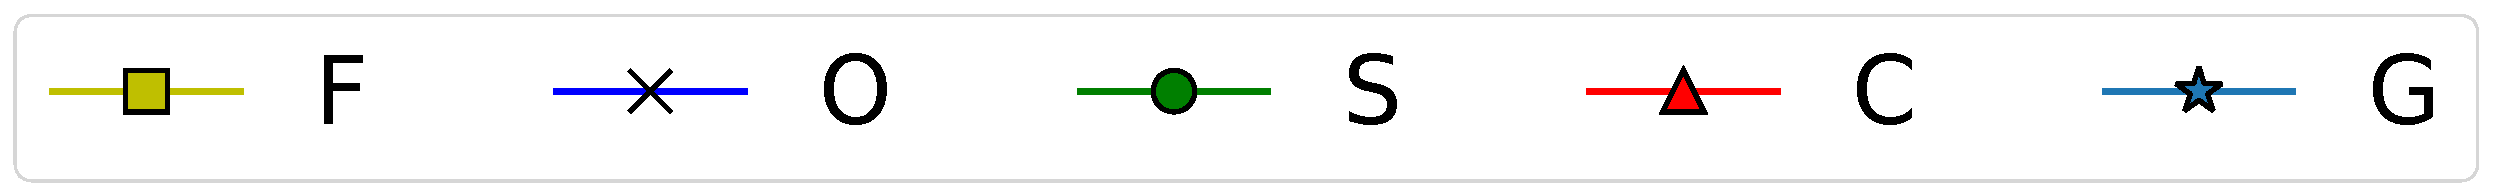
\includegraphics[width=0.4\linewidth]{fig/legend_f1}
	}
	\setcounter{subfigure}{0}
	\subfigure[Affects of Parameters on Different Events]{
		\label{fig:parameter_events}
		\begin{minipage}[b]{0.35\linewidth}
			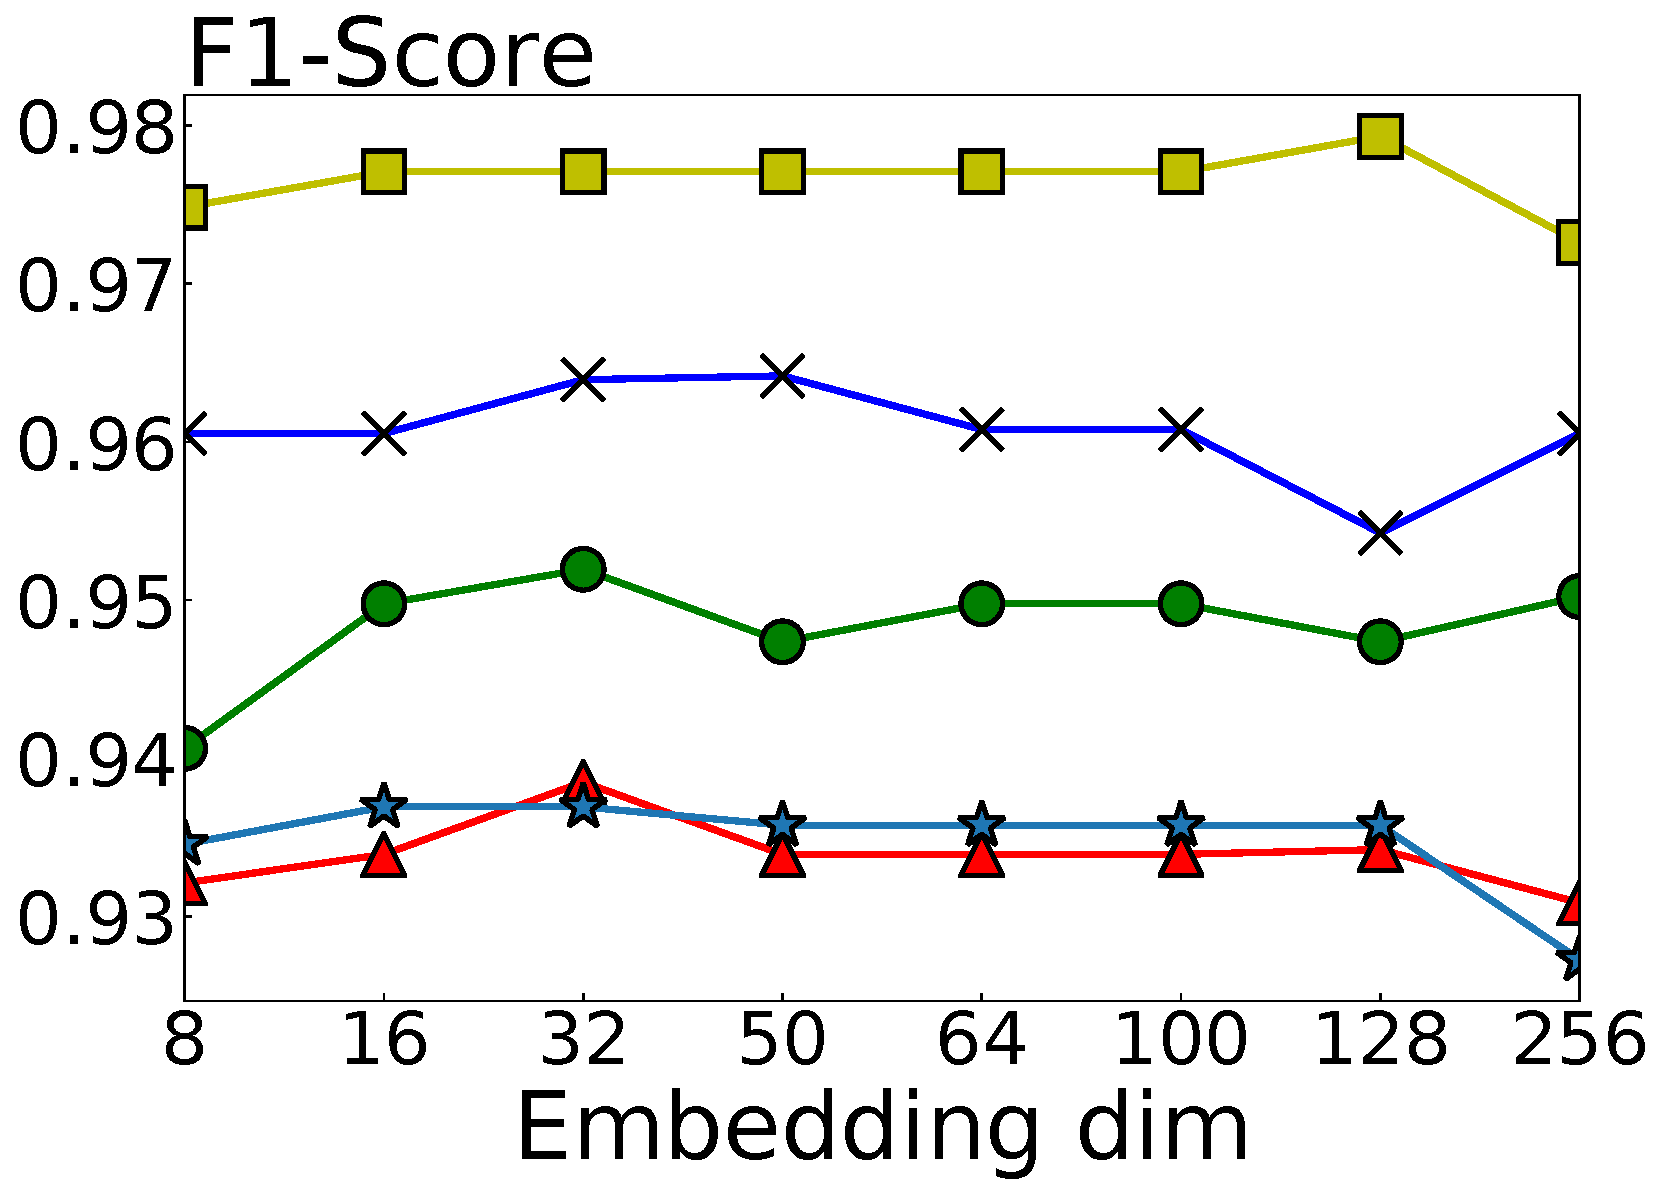
\includegraphics[width=1\linewidth]{fig/embedding_dim_events}
		\end{minipage}
		\begin{minipage}[b]{0.35\linewidth}
			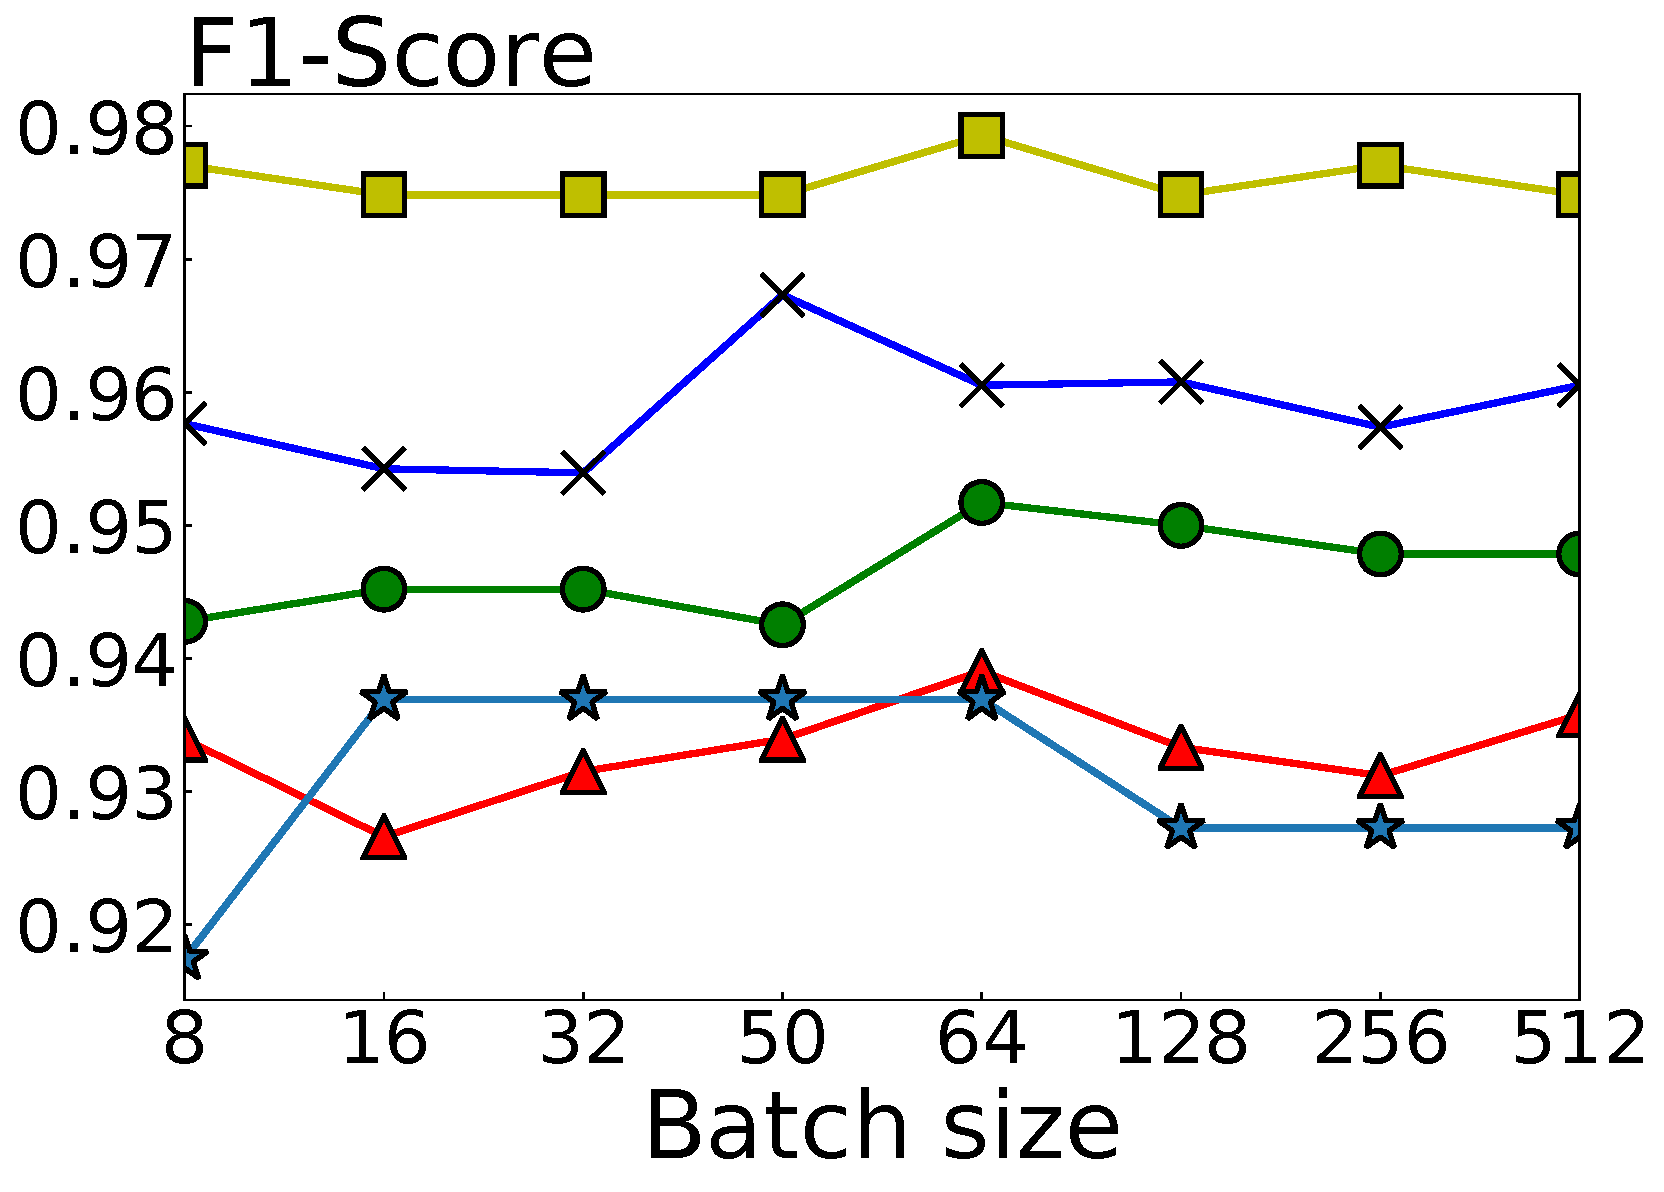
\includegraphics[width=1\linewidth]{fig/batch_size_events}
		\end{minipage}
		\begin{minipage}[b]{0.35\linewidth}
			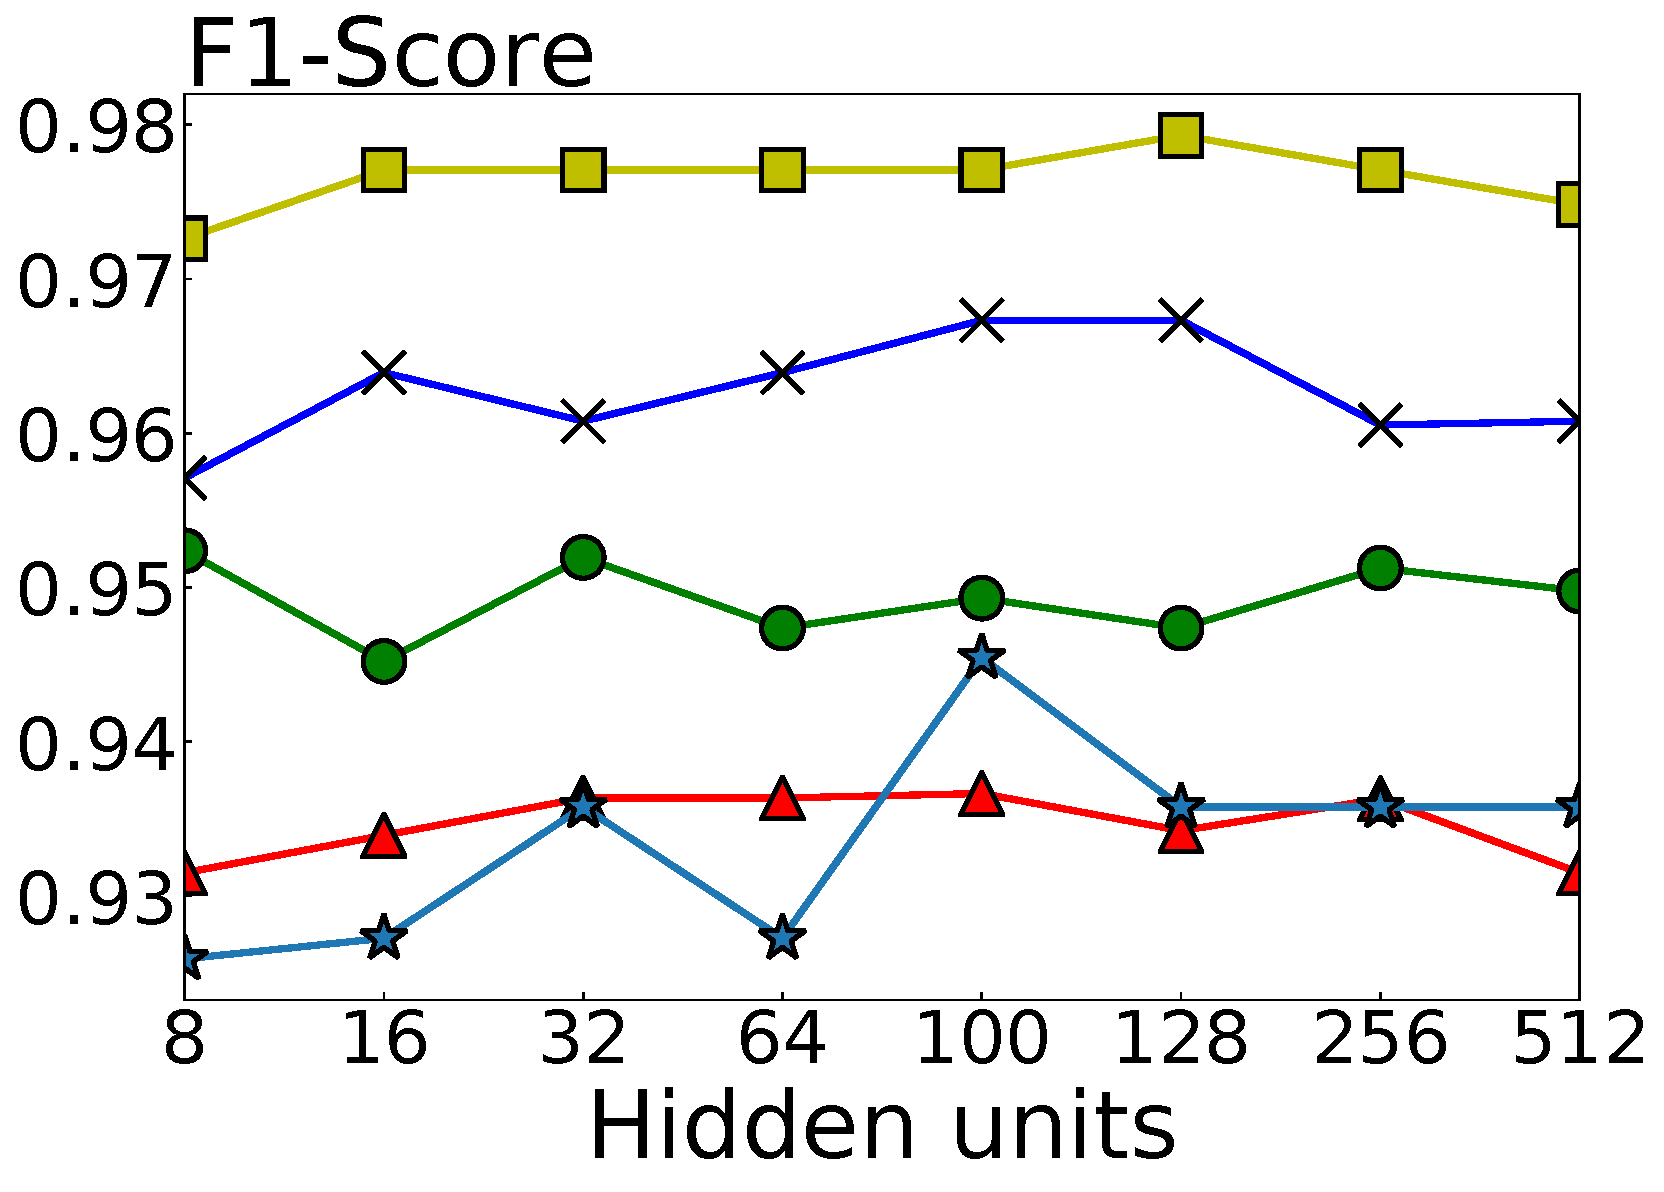
\includegraphics[width=1\linewidth]{fig/hidden_units_events}
		\end{minipage}
	}
	
	
	\subfigure{
		
\includegraphics[width=0.4\linewidth]{fig/legend_acc_macroF}
	}
	\setcounter{subfigure}{1}
	\subfigure[Affects of Parameters on Macro F1-Scores and Accruancy]{
		\label{fig:parameter_art}
		\begin{minipage}[b]{0.35\linewidth}
			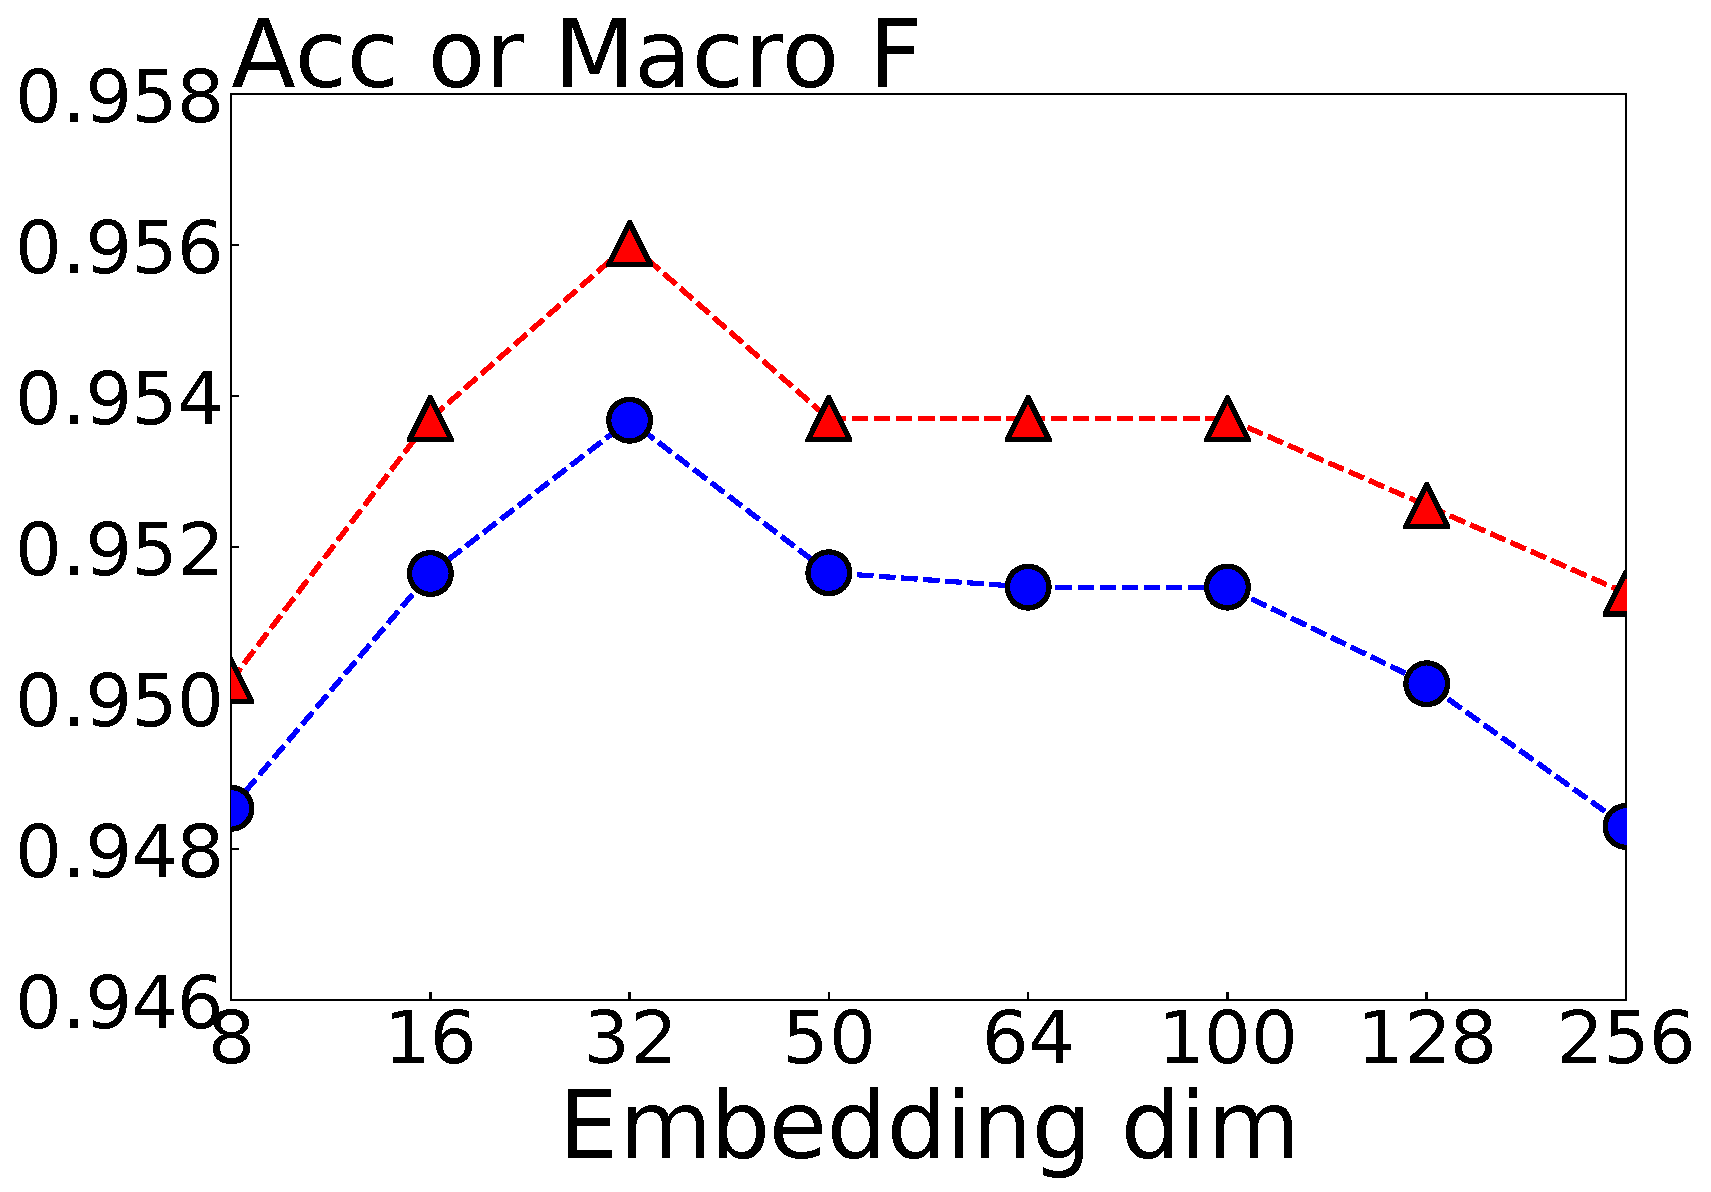
\includegraphics[width=1\linewidth]{fig/embedding_dim}
		\end{minipage}
		\begin{minipage}[b]{0.35\linewidth}
			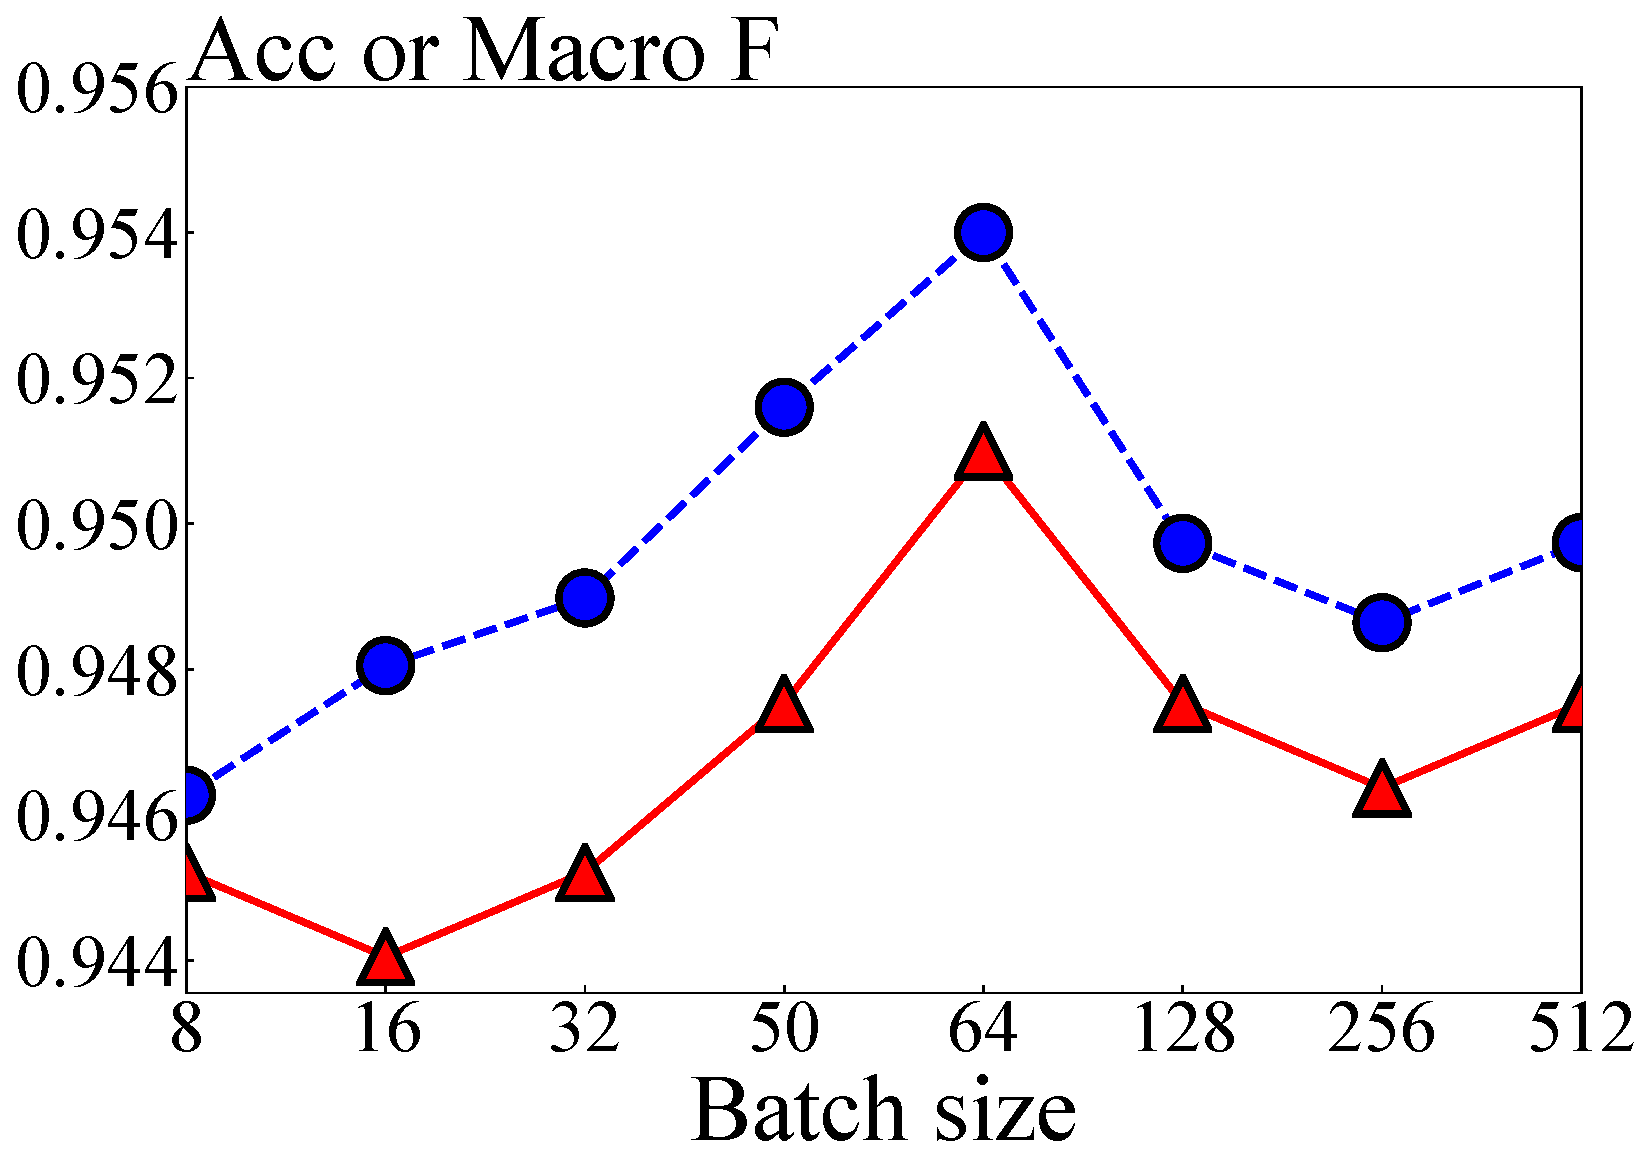
\includegraphics[width=1\linewidth]{fig/batch_size}
		\end{minipage}
		\begin{minipage}[b]{0.35\linewidth}
			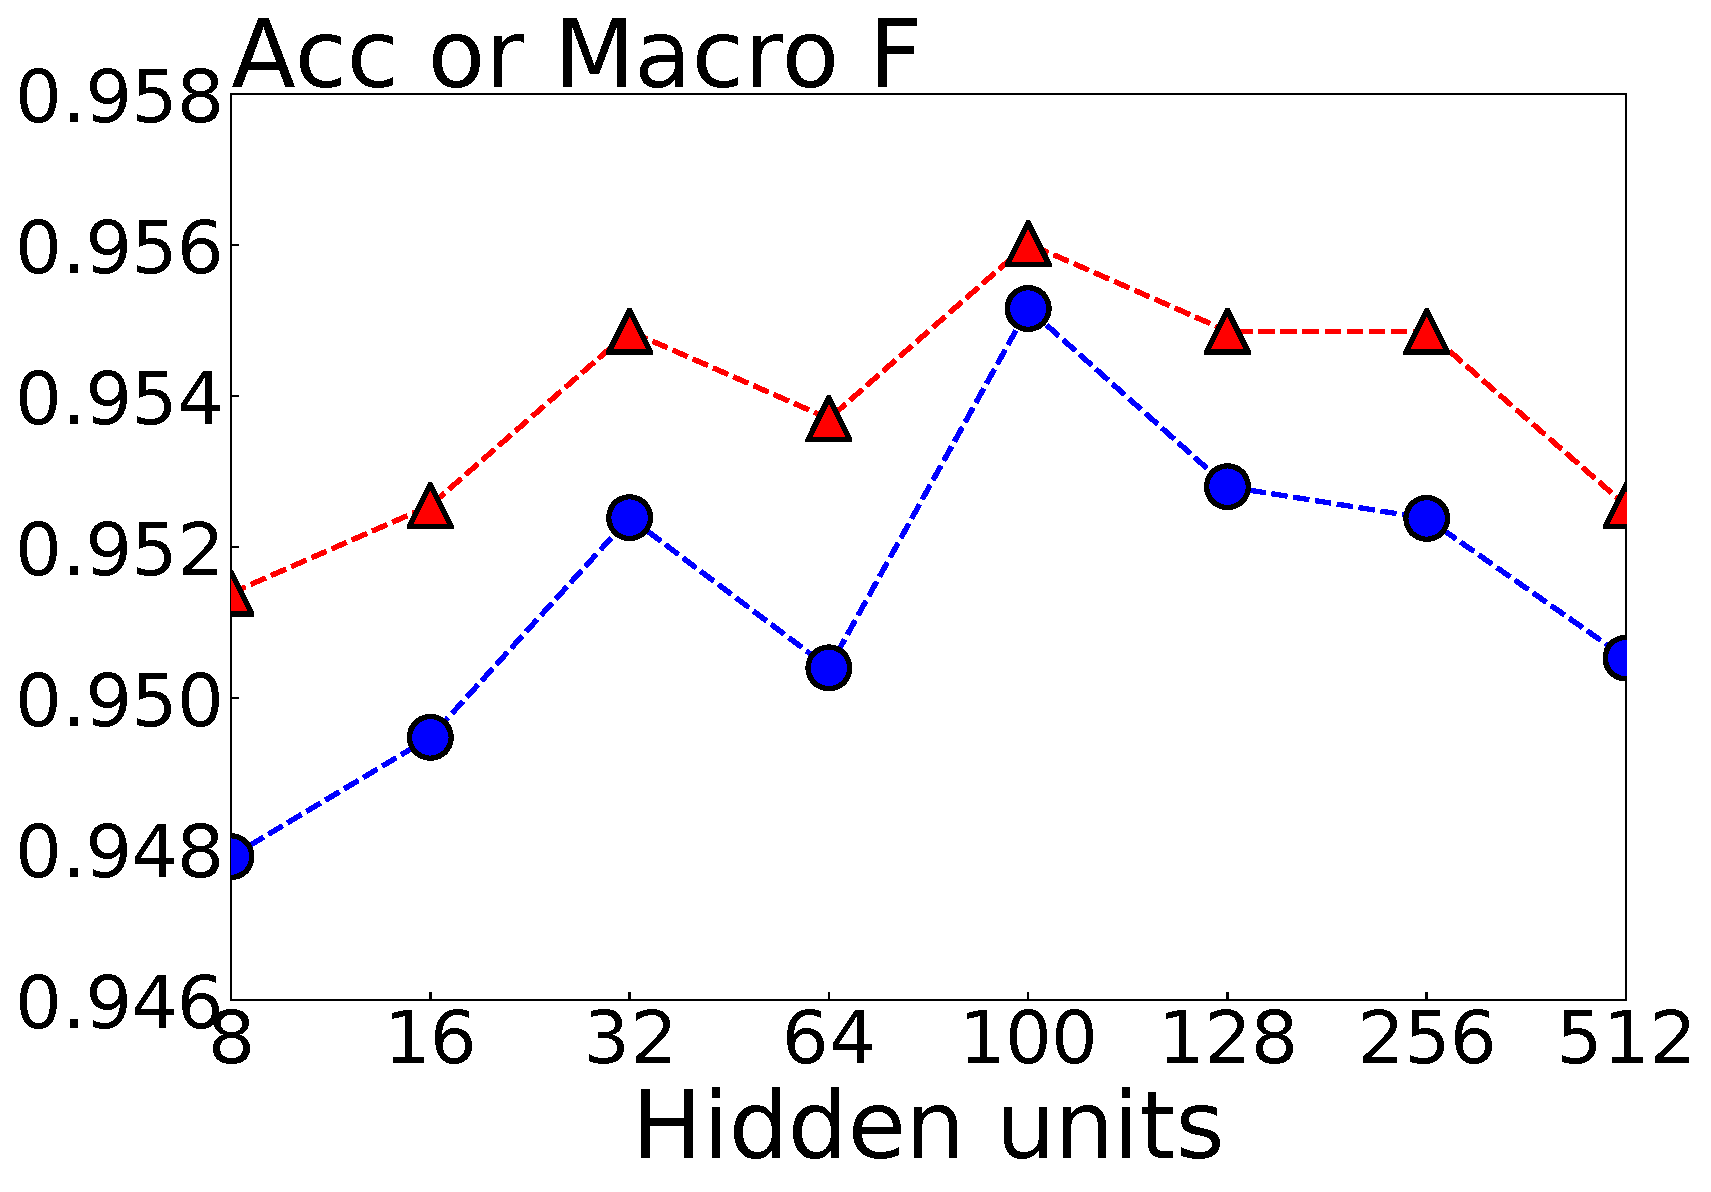
\includegraphics[width=1\linewidth]{fig/hidden_units}
		\end{minipage}
	}
	\caption{Adjustment of Parameters}
	\label{fig:parameter}
\end{figure}

\subsection{Details of Settings and Parameters}
In this part, we proceed to introduce the detailed settings of the experiments. The chosen optimizer in the deep learning based model is Adam. The loss function is cross-entropy. We split the whole dataset into a proportion of 6:2:2. For a deep learning based model, we run it more than 50 epochs until convergence. Besides, as shown in Fig.~\ref{fig:parameter}, we conduct various experiments to find the best parameters.

For simplicity, we only show the parameter adjustment on RumorEval as an example. We choose the embedding dimension, batch size, and hidden units as the representative parameters. During each running, we vary one parameter and fix the other parameters to record the variation trend of RL-BRT. The Fig.~\ref{fig:parameter_events} shows the results during parameter adjustment on each event. The Fig.~\ref{fig:parameter_art} records the performance of RL-BRT during parameter adjustment. It suggests that when the embedding dim is 32, batch size is 64, and hidden units are 100, RL-BRT achieves the best performance on RumorEval dataset. The smaller parameter value corresponds to the small scale of RumorEval.

\subsection{Discussion}
The experiments on baseline methods demonstrate the effectiveness of RL-BRT. RL-BRT outperforms the other models in most rumor events, showing robustness and superiority. The outstanding performance of the random embedding suggests that the pre-trained and the self-trained embeddings are not suitable in small-scaled dataset with causal spelling. Since some causal words are missing in pre-trained embeddings. Besides, the tweets are too short to train a satisfied self-trained embedding. The adjustment of the embedding dim shows that embeddings with small length is more suitable for rumor tracking. Because the long length embedding is spare, which brings additional computation. The comparison between the basic model, pairwise-added models, and RL-BRT further demonstrates the effectiveness of RL-BRT. 

